
%(BEGIN_QUESTION)
% Copyright 2014, Tony R. Kuphaldt, released under the Creative Commons Attribution License (v 1.0)
% This means you may do almost anything with this work of mine, so long as you give me proper credit

Beregn alle oppførte verdier for denne transformatorkretsen:

$$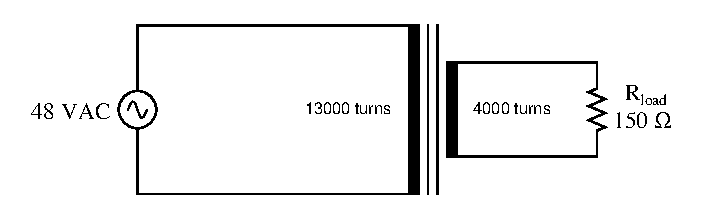
\includegraphics[width=15.5cm]{i01256x01.eps}$$

\begin{itemize}
\item{} $V_{primær} = $
\item{} $V_{sekundær} = $
\item{} $I_{primær} = $
\item{} $I_{sekundær} = $
\end{itemize}

Forklar om dette er en {\it opptransformator} (step-up), {\it nedtransformator} (step-down) eller {\it skilletransformator} (isolation), og forklar også hva som skiller ``primær''-viklingen fra ``sekundær''-viklingen i en hvilken som helst transformator.

\underbar{file i01256}
%(END_QUESTION)





%(BEGIN_ANSWER)

\begin{itemize}
\item{} $V_{primær} = 48 \hbox{ volt}$
\item{} $V_{sekundær} = 14.77 \hbox{ volt}$
\item{} $I_{primær} = 30.3 \hbox{ mA}$
\item{} $I_{sekundær} = 98.5 \hbox{ mA}$
\end{itemize}

Dette er en {\it nedtransformator}.

%(END_ANSWER)





%(BEGIN_NOTES)

De fleste transformatorproblemer er ikke noe mer enn forholdsregning, men noen studenter synes forhold er vanskelige å håndtere. Spørsmål som dette er flotte for å få studenter til å komme opp til tavlen foran i klasserommet og demonstrere hvordan de kom frem til resultatene.

%INDEX% Electronics review: transformer ratios

%(END_NOTES)
